% !TEX root = ../../Tesi_Triennale_PMNS.tex
\chapter[Algoritmo Coherent WaveBurst]{Coherent WaveBurst: algoritmo per la rivelazione e la ricostruzione di segnali di onde gravitazionali}
\label{chapter:cwb}
I dati forniti dalla rete di interferometri sono nella forma 
\[x(t) = \xi_k(t) + n(t)\]
dove $\xi_k(t)$ è la risposta del rivelatore al passaggio dell'onda gravitazionale, mentre $n(t)$ rappresenta il rumore di fondo dello strumento.
La risposta al segnale gravitazionale può essere scritta in una mappa tempo-frequenza come:
\begin{equation}
\xi_k = F_{+,k}h_+ + F_{\times,k}h_\times
\label{eqn:detector_response}
\end{equation}
dove $F_{+,k}(\theta,\phi)$ e $F_{\times,k}(\theta,\phi)$ sono gli antenna pattern del rivelatore k-esimo\cite{Klimenko_2008}. In particolare gli antenna pattern descrivono la risposta del detector al passaggio dell'onda gravitazionale e dipendono dalla posizione della sorgente nel cielo e dall'angolo di polarizzazione. 

Per semplicità si introduce la seguente notazione:
\[
\mathbf{x}[i,j] = \left(x_1[i,j],\dots, x_K[i,j] \right) ;
\quad
%\mathbf{w}[i,j] = \left(\frac{x_1[i,j]}{\sigma_1[i,j]},\dots, \frac{x_K[i,j]}{\sigma_K[i,j]} \right) ;
\]
\[
\mathbf{h}[i,j] = (h_+[i,j], h_\times[i,j])
\quad
\mathbf{f}_{+(\times)}[i,j] = \left(\frac{F_{1+(\times)}[i,j]}{\sigma_1[i,j]},\dots, \frac{F_{K+(\times)}[i,j]}{\sigma_K[i,j]} \right) 
\]
dove K è il numero di rivelatori nella rete, $x_k[i,j]$ è il campione di dati del rivelatore (l'indice $i$ itera sui tempi, mentre l'indice $j$ itera sulle frequenze)\cite{Klimenko_2008}, $h_{+}[i,j]$ e $h_{\times}[i,j]$ sono le ampiezze delle due polarizzazioni della GW. Si userà poi la notazione $\sum_{\Omega_{TF}} = \sum_{i,j=1}^N$, in quanto si scriverà $\Omega_{TF}$ come il dominio tempo-frequenza.

%Con le notazioni precedenti e denotando il rumore $\mathbf{n}[i,j]$, si può scrivere
%\begin{equation}
%\mathbf{x}[i,j] = \mathcal{F}\mathbf{h}[i,j] + \mathbf{n}[i]
%\end{equation}
%con $\mathcal{F}$ la matrice di antenna pattern, definita come
%%\begin{wrapfigure}{r}{0.46\textwidth}
%%	\vspace{-10pt}
%%	\begin{center}
%%		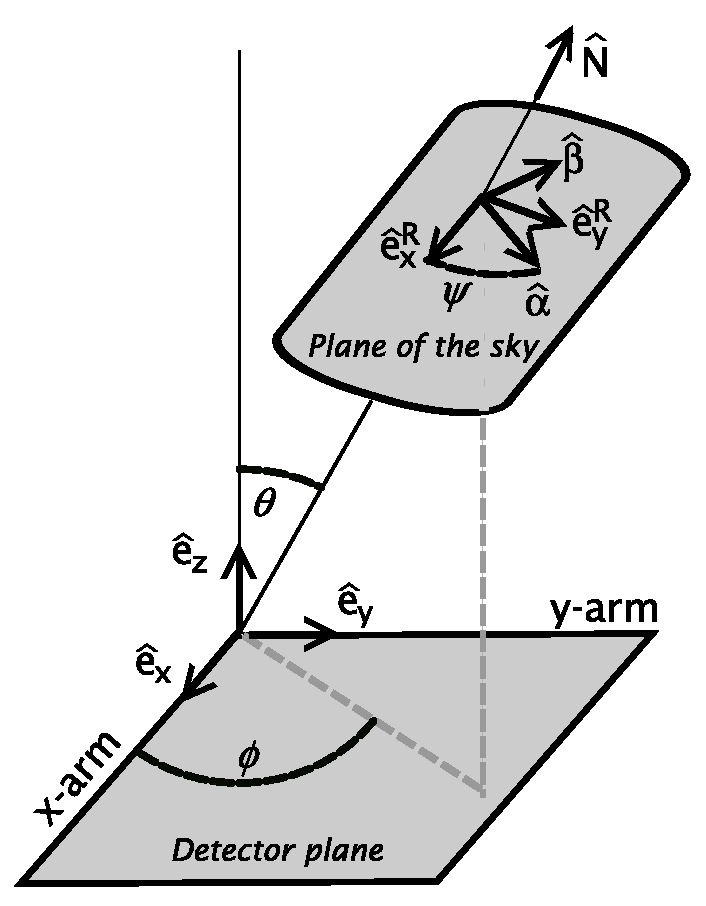
\includegraphics[width=0.25\textwidth]{figures/Capitolo_2/Detector_sky_full.eps}
%%	\end{center}
%%	\vspace{-5pt}
%%	\caption{L'orientazione relativa del piano delle polarizzazioni della GW e del piano su cui giacciono i bracci del detector, presa da \cite{Sathyaprakash_2009}.}
%%	\label{fig:antenna_pattern}
%%	\vspace{-30pt}
%%\end{wrapfigure}
%\begin{equation}
%\mathcal{F} = \begin{bmatrix}
%F_{1+}(\theta,\phi)	&F_{1\times}(\theta,\phi)\\
%\vdots					&   \vdots				 \\
%F_{K+}(\theta,\phi)	&F_{K\times}(\theta,\phi)\\
%\end{bmatrix}
%\end{equation}

%Gli antenna pattern descrivono come il detector riceve l'energia in funzione della posizione angolare e, in particolare, sono caratterizzati da una trasformazione basata sull'angolo di polarizzazione $\Psi$, equivalente alla rotazione del piano sul quale è definito $\mathbf{h}$.

%Nei metodi coerenti le statistiche vengono calcolate come somma coerente delle risposte dei detector singoli. Gli algoritmi che sfruttano questi metodi risultano più efficienti, devono cioè avere una probabilità di falso allarme più bassa, rispetto alle statistiche calcolate sulle risposte di ogni detector singolarmente.

L'algoritmo che si utilizza, Coherent WaveBurst (cWB), ricerca eccessi di potenza nella rappresentazione in un piano tempo-frequenza del segnale, coerenti fra i rivelatori attraverso l'utilizzo di una statistica coerente costituita da una analisi della massima verosimiglianza.\\
%L'algoritmo differisce dai metodi tradizionali che identificano gli eventi nei detector singolarmente usando statistiche di eccesso di potenza e poi verificano la coerenza tra i segnali nei vari detector.
L'utilizzo di una statistica costruita coerentemente fra le risposte degli interferometri si dimostra più efficiente dei metodi che impongono la sola coincidenza temporale fra i segnali degli interferometri. Infatti si avranno molteplici vantaggi: innanzitutto la sensibilità del metodo non sarà limitata dal rivelatore meno sensibile nella rete, in quanto la likelihood utilizzata nei metodi coerenti rappresenta il rapporto segnale su rumore (SNR) totale del segnale ricostruito/rivelato dalla rete. 
Inoltre questo metodo permette di costruire altre statistiche coerenti, come il coefficiente di correlazione fra i rivelatori e la stima della componente coerente e non coerente, per distinguere segnali che effettivamente hanno una controparte fisica rispetto a eccessi di rumore ambientale o strumentale. Infine, è possibile ricostruire la posizione celeste della sorgente\cite{Klimenko_2008}.

L'algoritmo cWB viene utilizzato all'interno della collaborazione LIGO-Virgo sia per l'analisi dei segnali in bassa latenza, per identificare e ricostruire candidati significativi e poter, una volta ottenuta una prima stima della posizione celeste della sorgente, condividerla con i telescopi partner per identificare i segnali elettromagnetici legati; sia per l'analisi di dati consolidati, volta a ottenere risultati più approfonditi sull'evento, stabilendo la significanza degli eventi osservati e identificando le stelle progenitrici\cite{Klimenko_2016}.
\section{Metodologia di analisi per la ricerca di segnali gravitazionali}
\label{section:coherent_analysis}
Per rivelare e ricostruire segnali, la pipeline di cWB utilizza un metodo basato sul rapporto di verosimiglianza, definito come il logaritmo del rapporto di verosimiglianza
\begin{equation}
	\Lambda(\mathbf{x},\Omega) = \frac{p(\mathbf{x}|\mathbf{h}(\Omega))}{p(\mathbf{x}|0)}
\end{equation}
dove $\Omega$ è il set di parametri che descrive il segnale, $p(\mathbf{x}|0)$ è la probabilità dell'ipotesi nulla $H_0$, quindi di solo rumore strumentale, mentre $p(\mathbf{x}|\mathbf{h})$ è la probabilità dell'ipotesi alternativa $H_1$, ovvero la probabilità composta che vi sia un segnale $\mathbf{h}$ nel campione $\mathbf{x}$\cite{Klimenko_2016}.


Nell'ipotesi idealistica di rumore gaussiano quasi stazionario con deviazione standard $\sigma$ le densità di probabilità associate alle ipotesi $H_0$ e $H_1$ in un piano tempo-frequenza sono 
\begin{equation}
	p(x|0)) = \prod_{i=1}^N\frac{1}{\sqrt{2\pi}\sigma^2}\exp(-\frac{x^2[i,j]}{2\sigma^2})
	\quad\quad
	p(x|h(\Omega)) = \prod_{i=1}^N\frac{1}{\sqrt{2\pi}\sigma^2}\exp(-\frac{(x[i,j]-\xi[i,j])^2}{2\sigma^2}).
\end{equation}
Il funzionale di verosimiglianza può essere scritto quindi come
\begin{equation}
	L = \ln(\Lambda(x)) = \sum_{i=1}^{N}\left[\frac{1}{\sigma^2}\left(x[i,j]\xi[i,j]-\frac{1}{2}\xi^2[i,j]\right)\right].
\end{equation}
Estendendo ad una rete di K rivelatori, supponendo rumore scorrelati tra i vari rivelatori, si scriverà
\begin{equation}
	\mathcal{L} = \sum_{k=1}^{K}\sum_{i,j=1}^{N}\left(\frac{x_k^2[i,j]}{\sigma_k^2[i,j]} - \frac{(x_k[i,j]-\xi_k[i,j])^2}{\sigma_k^2[i,j]}  \right)
	\label{eqn:Likelihood}
\end{equation}

Il rumore del rivelatore è caratterizzato dalla deviazione standard $\sigma_k[i,j]$,  anch'essa una funzione sul piano tempo-frequenza. 
%I valori saranno i dati scalati con il rumore (detti sbiancati)\cite{Klimenko_2016}. 

Dunque, al variare di $h_{+}[i,j]$ e $h_{\times}[i,j]$ varia anche $\mathcal{L}$, l'obiettivo è quindi massimizzare il rapporto di verosimiglianza, al variare della possibile posizione nel cielo del segnale. Il segnale viene alla fine ricostruito tramite una trasformazione wavelet inversa nella posizione di massimizzazione della verosimiglianza
%l'obiettivo è quindi ottenere i valori delle ampiezze che massimizzano il funzionale di verosimiglianza da cui si deduce la forma d'onda nel dominio dei tempi facendo una trasformazione di wavelet inversa.%, che consisterà dunque 

Il funzionale rapporto di verosimiglianza in equazione \ref{eqn:Likelihood} si può scrivere come
\begin{equation}
%	\mathcal{L} = \braket{w}{\xi} - \frac{1}{2} \braket{\xi}{\xi} = \mathcal{L}_+ + \mathcal{L}_\times = \sum_{\Omega_{TF}}\left[ \mathbf{w} \cdot \mathbf{f}_+ - \frac{1}{2}|\mathbf{f}_+|^2h_+^2\right] + \sum_{\Omega_{TF}}\left[ \mathbf{w} \cdot \mathbf{f}_\times - \frac{1}{2}|\mathbf{f}_\times|^2h_\times^2\right]
	\mathcal{L} =  \mathcal{L}_+ + \mathcal{L}_\times = \sum_{\Omega_{TF}}\left[ \mathbf{w} \cdot \mathbf{f}_+ - \frac{1}{2}|\mathbf{f}_+|^2h_+^2\right] + \sum_{\Omega_{TF}}\left[ \mathbf{w} \cdot \mathbf{f}_\times - \frac{1}{2}|\mathbf{f}_\times|^2h_\times^2\right]
	\label{eqn:label_separated}
\end{equation}
dove i vettori di antenna pattern $\mathbf{f}_+$ e $\mathbf{f}_\times$ sono definiti nel Dominant Polarisation wave Frame (DPF), ovvero il piano in cui entrambi gli antenna pattern sono reali, definiti positivi e vale $\mathbf{f}_+ \cdot \mathbf{f}_\times = 0$.  Alla luce di questo, per ottenere la massima verosimiglianza si dovrà risolvere le equazioni:
\begin{equation}
%	\mathbf{w} \cdot \mathbf{f}_+ = |\mathbf{f}_+|^2h_+ \quad\quad\quad  \mathbf{w} \cdot \mathbf{f}_\times = |\mathbf{f}_+|^2h_\times 
	\begin{bmatrix}
	(\mathbf{w}[i,j]\cdot \mathbf{e}_+[i,j])\\
	(\mathbf{w}[i,j]\cdot \mathbf{e}_\times[i,j])
	\end{bmatrix}
	=
	\begin{bmatrix}
	\mathbf{f}_+[i,j]	&0\\
	0					&\mathbf{f}_\times[i,j]
	\end{bmatrix}
	\begin{bmatrix}
	h_+[i,j]\\
	h_\times[i,j]\\
	\end{bmatrix}
	\label{eqn:sistema_soluzione}
\end{equation}
%La massima verosimiglianza può essere scritta quindi sostituendo le soluzioni di \ref{eqn:sistema_soluzione} in $\mathcal{L}(h)$, che restituisce
%\begin{equation}
%	L_{max} = \sum_{\Omega_{TF}}\mathbf{w}[i,j]P[i,j]\mathbf{w}^\intercal[i,j]
%\end{equation}
%dove la matrice $P$ è il proiettore costruito a partire dai versori $\mathbf{e}_+$ e $\mathbf{e}_\times$:
%\begin{equation}
%	P_{nm}[i,j]=e_{n+}[i,j]e_{m+}[i,j]+e_{n\times}[i,j]e_{m\times}[i,j]
%	\label{eqn:proiection}
%\end{equation}

%\paragraph{Regolatori} C'è una particolare classe di vincoli, i regolatori, che dipendono da come il network reagisce a un determinato segnale. Si può citare un esempio considerando il caso in cui $|f_\times|=0$, come nel caso di detector allineati; la risposta del network dovrebbe essere lungo la direzione di $f_+$ e imporre questo vincolo porta l'analisi della likelihood a ignorare la risposta-$\times$ del network. Anche per detector non allineati si utilizzano questo tipo di vincoli: in base alla posizione della sorgente, il network può essere meno sensibile alla seconda componente della GW ($|\mathbf{f}_\times|^2 \ll |\mathbf{f}_+|^2$) portando a problemi nella ricostruzione di $h_\times$. Quello che viene fatto da cWB è cambiare la norma di $\mathbf{f}_\times$ con un parametro $\delta$, equivalente ad aggiungere un ulteriore detector al network che permette di preservare l'ortogonalità di $\mathbf{e}_+ \text{ e } \mathbf{e}_\times'$.
\section{Algoritmo cWB}
L'algoritmo, scritto in C++/ROOT e sviluppato all'interno della collaborazione LIGO-Virgo, ha la caratteristica di non imporre assunzioni (o facendo assunzioni minimali) sulla morfologia del segnale.\\
Vengono descritti i principali step dell'algoritmo: trasformazione di wavelet, generazione di trigger coerenti e selezione dei trigger coerenti.
\subsection{Rappresentazione in tempo-frequenza}
\begin{wrapfigure}{r}{0.46\textwidth}
	\vspace{-15pt}
	\begin{center}
		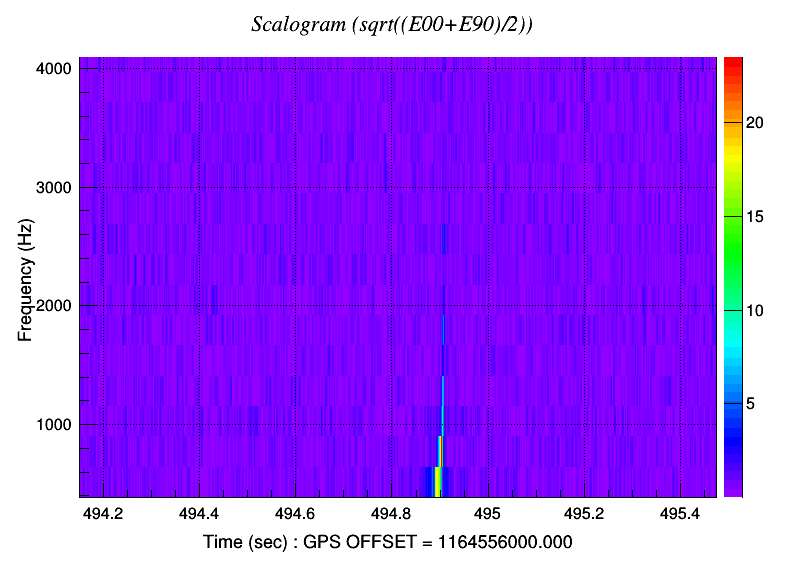
\includegraphics[width=0.475\textwidth]{figures/Capitolo_2/L1_scalogram_0.png}
	\end{center}
	\vspace{-5pt}
	\caption{Scalogramma ottenuto da una analisi di una simulazione di coalescenza di una BNS con EOS SHT2.0 con rumore gaussiano del rivelatore LIGO Hanford, con risoluzione df = 256kHz e dt = 2ms}
	\label{fig:scalogram_example}
	\vspace{-15pt}
\end{wrapfigure}
\label{subsection:wavelet_transform}
Le trasformazioni di wavelet, partendo dai dati discreti, producono rappresentazioni tempo-frequenza dei dati dei rivelatori $w[i,j]$. Lo spettro di wavelet può essere quindi rappresentato con uno scalogramma tempo-frequenza. La risoluzione nel dominio del tempo $\Delta t_j(R)$ è determinata dal rate di campionamento R e dall'indice di scala j. Poiché le trasformazioni di wavelet costituiscono una serie di trasformazioni di Fourier infinitesime, conservano il volume del campione, pari a 1/2 per la serie temporale in input.\\
Si avrà quindi una risoluzione in frequenza $\Delta f_j$ definita come 1/(2$\Delta t_j$) che determina la larghezza di banda per l'indice j. Per ottimizzare la ricerca nel piano, cWB procede con diverse trasformazioni a risoluzioni diverse, che permette di ottenere il grafico in Figura \ref{fig:scalogram_example}\cite{Klimenko_2008}.

I valori nella mappa tempo-frequenza vengono sbiancati: partendo dalla mappa con massima risoluzione in frequenza per ogni banda di frequenza viene calcolato il valore di scarto quadratico medio del rumore, utilizzando una media mobile. Quindi i dati nel piano tempo-frequenza sono normalizzati rispetto allo scarto quadratico medio e scalati con il rumore come $w_k[i,j] = x_k[i,j]/\sigma_k[i,j]$ \cite{Klimenko_2016}.

\begin{wrapfigure}{r}{0.46\textwidth}
	\vspace{-15pt}
	\begin{center}
		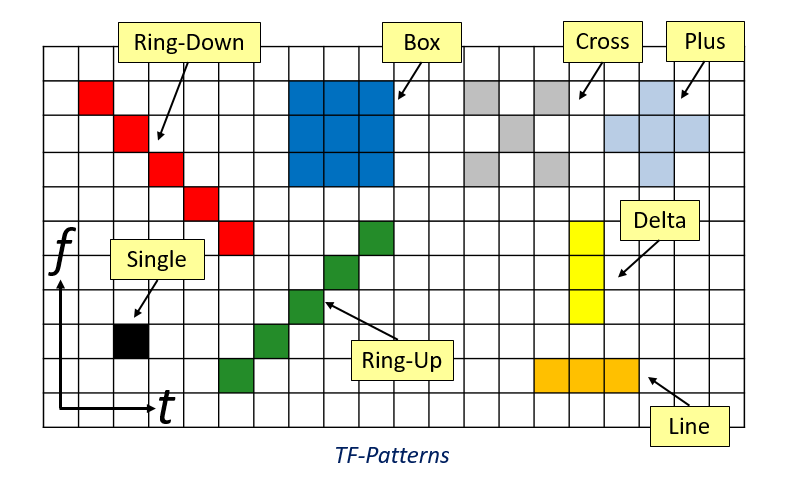
\includegraphics[width=0.475\textwidth]{figures/Capitolo_2/wavepacket_patterns.png}
	\end{center}
	\vspace{-5pt}
	\caption{Alcuni pattern caratteristici per la selezione dei pixel}
	\label{fig:patterns}
	\vspace{-15pt}
\end{wrapfigure}
cWB esegue trasformazioni di wavelet a diverse risoluzioni e per ogni risoluzione seleziona i pixel con eccesso di potenza che saranno selezionati per il prossimo passo dell'analisi. I pixel con eccesso di potenza vengono scelti se superano una soglia definita. Tale soglia fa riferimento alla coda destra di probabilità di una distribuzione gaussiana attesa per il rumore. Infine, poiché un evento deve essere costituito da un gruppo di pixel contigui, vengono selezionati i gruppi pixel che soddisfano diverse possibili condizioni sull'eccesso di potenza rispetto alla media attesa per il rumore \cite{cWB_Manual}. Si riportano in Figura \ref{fig:patterns} alcuni dei pattern di selezione di cWB.
%\subsection{Filtro di predizione lineare dell'errore}
%\label{subsection:lpe_filter}
%I filtri per la predizione lineare dell'errore (LPE) sono usati per rimuovere le componenti prevedibili dalla serie temporale in input. Possono essere applicati nel dominio di wavelet, ma più frequentemente vengono usati nel dominio temporale restituendo una serie temporale sbiancata.
%
%Ogni layer di wavelet (quindi a frequenza fissata) è una serie temporale, perciò anzichè applicare il filtro LPE alla sere temporale $x(t)$, si può fare prima una decomposizione di wavelet $x(t)\rightarrow w(f,t)$ e quindi applicare il filtro ad ogni layer di wavelet. Si ottiene dunque un campione $w'(f, t)$ da cui è possibile ricostruire la serie temporale sbiancata $x'(t)$ attraverso una trasformazione di wavelet inversa\cite{Klimenko_2008}.
%\subsection{Filtri per il ritardo temporale nel dominio di wavelet}
%\label{subsection:time_delay_filters}
%Per la valutazione della likelihood è necessario computare il prodotto scalare $\bra{x_n(\tau_n)}\ket{x_m(\tau_m)}$, dove bisogna considerare un ritardo intrinseco del set di dati del rivelatore $n$ rispetto a $m$, in quanto le GW viaggiano a velocità finita pari a $c$. Dunque il ritardo temporale $\tau_n - \tau_m$ dipende dalla posizione $(\theta, \phi)$ della sorgente.
%
%Nel dominio di wavelet è invece necessario calcolare il prodotto interno $\bra{w_n(\tau_n)}\ket{w_m(\tau_m)}$, le ampiezze ritardate possono essere calcolate a partire dalle ampiezze originali utilizzando un filtro di ritardo temporale $D_{kl}(\tau)$
%\begin{equation}
%	w_{n,m}(i,j,\tau) = \sum_{kl}D_{kl}(\tau, j)w_{n,m}(i+k, j+l)
%	\label{eqn:time_filter}
%\end{equation}
%dove $k$ ed $l$ sono le coordinate locali nel piano tempo-frequenza rispetto alla posizione $(i,j)$.
%
%La costruzione di questi filtri è legata alla decomposizione delle funzioni di wavelet ritardate $\Psi_j(t+\tau)$ nella base delle funzioni non traslate $\Psi_j(t)$. Si procede dunque per step:
%\begin{enumerate}
%	\item viene creata una serie di wavelet con un solo coefficiente pari all'unità nella posizione $(i,j)$;
%	\item viene applicata la trasformazione di wavelet inversa ricostruendo $\Psi_j(t)$ nel dominio dei tempi;
%	\item viene applicata la traslazione temporale $\Psi_j(t)\rightarrow\Psi_j(t+\tau)$ e si decompone quest'ultima;
%	\item le ampiezze di wavelet ottenute nelle posizioni $(i+k, j+l)$ rappresentano i coefficienti del filtro $D_{kl}(\tau, j)$ per il layer j.
%\end{enumerate}
%L'applicazione di questo filtro porta a una perdita di energia, valutabile in $\epsilon_K = 1 - \sum_{K}D_{kl}^2$
%%\begin{equation}
%%	\epsilon_K = 1 - \sum_{K}D_{kl}^2
%%	\label{eqn:energy_loss}
%%\end{equation}
%e perciò la lunghezza del filtro sarà legata alla quantità di energia acsecettabile da perdere (valori tipici sono $K>20$ per ottenere una perdita di energia inferiore a $1\%$)\cite{Klimenko_2008}.
\subsection{Generazione di trigger coerenti}
\label{section:coherent_trigger}

La generazione dei trigger, quindi l'identificazione dei segnali, è basata su statistiche di eccesso di potenza e di correlazione incrociata tra i segnali dei rivelatori. 

\begin{wrapfigure}{r}{0.46\textwidth}
	\vspace{-25pt}
	\begin{center}
		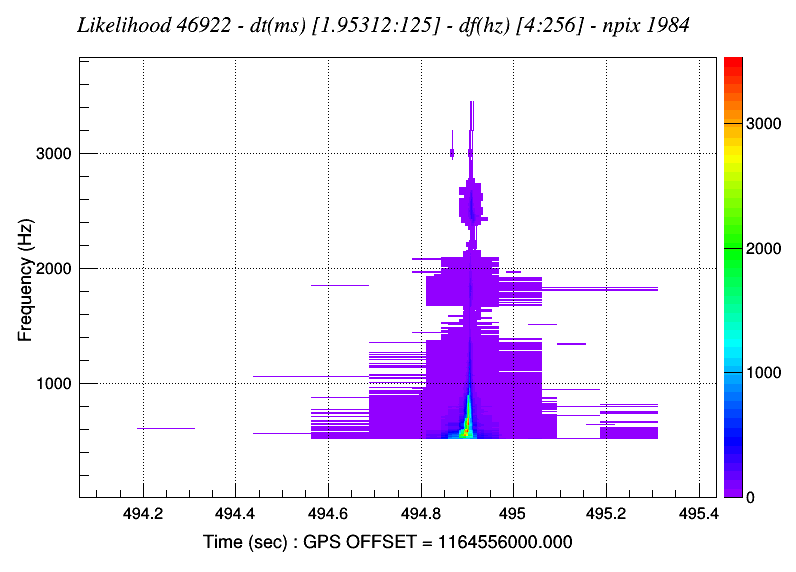
\includegraphics[width=0.475\textwidth]{figures/Capitolo_2/l_tfmap_scalogram.png}
	\end{center}
	\vspace{-5pt}
	\caption{Mappa di Likelihood ottenuta da una analisi di una simulazione di coalescenza di una BNS con EOS SHT2.0 con rumore gaussiano della rete LIGO-Virgo}
	\label{fig:Likelihood_example}
	\vspace{-10pt}
\end{wrapfigure}
Riprendendo quanto scritto in \ref{eqn:Likelihood}, il funzionale di likelihood viene calcolato come somma sui campioni selezionati per l'analisi, il numero di termini sommati dipende all'area nel piano tempo-frequenza che si considera. Se tale somma consiste di un solo elemento si può scrivere il funzionale come
\begin{equation}
	\mathcal{L}_p(i,j,\theta,\phi)=|\mathbf{w}|^2 -|\mathbf{w} - \mathbf{f}_+h_+ - \mathbf{f}_\times h_\times|^2
	\label{eqn:likelihood_single_term}
\end{equation}
Poiché è possibile applicare il metodo della likelihood al funzionale \ref{eqn:likelihood_single_term}, si può trovare il massimo $L_p(\theta, \phi)$ al variare di $h_+$ e $h_\times$ e quindi ricercare il massimo in funzione della posizione nel cielo
\begin{equation}
	L_m(i,j)= \max_{\theta, \phi}[L_p(i,j,\theta,\phi)]
	\label{eqn:max_L}
\end{equation}
La statistica $L_m$ ha quindi il significato della massima energia rivelata dalla rete in una determinata posizione del piano tempo-frequenza. Selezionando quindi i valori di $L_m$ sopra una determinata soglia si può identificare un cluster di pixel come potenziale segnale di GW. In questo modo si identificano i segnali combinando i dati dell'intera rete e non si cercano i segnali sui singoli rivelatori, verificando successivamente la coerenza.
%A questo punto si devono ricostruire i parametri del segnale legato al trigger, incluse la posizione della sorgente, le due polarizzazioni della GW, le risposte individuali dei rivelatori e le statistiche di massima likelihood dei trigger. In particolare la likelihood è ricostruita come
%\begin{equation}
%	\mathcal{L}_c(\theta,\phi) = \sum_{i,j}\mathcal{L}_p(i,j,\theta, \phi)
%\end{equation}
%La massima likelihood $L_{max}$ è ottenuta facendo variare $\mathcal{L}_c$ su $\theta$ e $\phi$ ed è calcolata su tutti i pixel di likelihood nel piano tempo frequenza per formare il trigger coerente\cite{Klimenko_2008}.
\subsection{Selezione dei trigger coerenti}
Nel caso di rumore gaussiano stazionario la massima verosimiglianza è l'unica statistica necessaria per la rivelazione e per la selezione degli eventi, per cui la probabilità di falso allarme e di scartare eventi effettivi è legata alla soglia minima per $L_{max}$. 
%Nella realtà tuttavia il rumore non è tale, ma i dati sono sporcati da rumore strumentale e ambientale, per cui è necessario applicare altri metodi per distinguere i segnali reali. 
La condizione di idealità non si realizza nella realtà, motivo per cui cWB utilizza estimatori sulla coerenza del segnale per distinguere possibili segnali gravitazionali, da eccessi di rumore strumentale e ambientale.
Alcuni esempi sono le statistiche coerenti ricavate dalle matrici di verosimiglianza e di energia non coerente.
La matrice di likelihood $L_{mn}$ è ottenuta dalla forma quadratica della likelihood
%da completare la parte dei regolatori a cui questa parte fa riferimento.
\begin{equation}
	L_{max} = \sum_{mn}L_{mn} = \sum_{mn}\left[\left< w_nw_me_{+n}e_{+m} \right> + \left< w_nw_me_{\times n}e_{\times m} \right>\right]
	\label{eqn:likelihood_matrix}
\end{equation}
dove $m\text{ e }n$ sono gli indici che identificano i rivelatori\cite{Klimenko_2008}. Gli elementi della diagonale di $L_{mn}$ descrivono l'energia incoerente normalizzata, mentre quelli dell'antidiagonale sono espressione dell'energia coerente normalizzata, la cui somma restituisce l'energia coerente totale $E_{coh}$ rivelata dalla rete
\begin{equation}
	E_{inc} = \sum_{\Omega_{TF}}\sum_{n}w_n[i,j]P_{mn}[i,j]w_n[i,j],
	\quad\quad
	E_{coh} = \sum_{\Omega_{TF}}\sum_{m\neq n}w_n[i,j]P_{mn}[i,j]w_n[i,j].
\end{equation}
dove la matrice $P$ è il proiettore costruito a partire dai versori $\mathbf{e}_+$ e $\mathbf{e}_\times$: $P_{nm}[i,j]=e_{n+}[i,j]e_{m+}[i,j]+e_{n\times}[i,j]e_{m\times}[i,j]$\cite{Klimenko_2016}. 
%Queste statistiche coerenti sono particolarmente utilizzate per la ricerca di segnali e la ricostruzione.
%Si può dunque esprimere i coefficienti di correlazione per detector allineati e quindi l'energia coerente ridotta
%\begin{equation}
%	r_{mn} = \frac{L_{mn}}{\sqrt{L_{nn}L_{mm}}} \quad\quad\quad \rightarrow \quad\quad\quad e_{coh}=\sum_{ n\neq m}L_{nm}|r_{nm}|
%	\label{eqn:coherent_energy}
%\end{equation}
%quest'ultima in particolare risulta uno dei parametri più efficienti per l'accettazione/rifiuto di un trigger.

La matrice di energia non coerente rappresenta l'energia normalizzata del rumore ricostruito
\begin{equation}
	N_{nm} = E_{nm}-L_{nm}
\end{equation}
con $E_{mn}$  matrice diagonale delle energie normalizzate dei rivelatori $E_{mm}  = \left<x_m^2\right>$. Per distinguere i segnali effettivi dal rumore strumentale e ambientale si usano i coefficienti di correlazione 
\begin{equation}
	C_{net} = \frac{E_{coh}}{N_{ull}+|E_{coh}|}, \quad\quad\quad c_{net} = \frac{e_{coh}}{N_{ull}+|e_{coh}|}
	\label{eqn:coefficient_energy}
\end{equation}
dove $N_{ull}$ è la somma di tutti gli elementi della matrice di non coerenza, che rappresenta l'energia totale non coerente. Accade infatti che eccessi di rumore vengano ricostruiti come segnale: i coefficienti $C_{net}$ e $c_{net}$ sono usati quindi come verifica della consistenza del segnale in quanto comparano l'energia non coerente e l'energia coerente\cite{Klimenko_2008}, in particolare un evento genuino risulta per $c\smallsim 1$, mentre per $c \ll 1$ corrisponde ad un evento spurio\cite{Klimenko_2016}.